\documentclass[a4paper]{scrartcl}
\usepackage[cm]{fullpage}
\usepackage{amsmath, amssymb, esint}
\usepackage{siunitx}
\usepackage{caption}

\usepackage{tikz}

\begin{document}

\title{PHYS2111: Double Slit Interference}
\author{ \\ \\ }
\date{2016-04-27}
\maketitle

\section{Introduction}
Please refer to the student notes of the experiment.

\section{Materials and Methods}
Please refer to the operating instructions and prework of the experiment.

The values for the slit width (\(W = \SI{0.085}{\milli\metre}\)) and slit centre-to-centre distance (\(d = \SI{0.457}{\milli\metre}\)) given in the operating instructions were assumed to be correct with uncertainty below the specified precision. The double slit to detector slit distance was measured to be \(L = \SI{500 \pm 2}{\milli\metre}\).

The laser used for the wave mode was red in colour, while the bulb light used for the particle mode was green, but both of unknown wavelength.

All single slit measurement were taken with the right slit of the double slit.

During the particle mode of the experiment, the recommend ``5'' setting resulting in an maximum reading too close to dark current for comfort (\(\approx\SI{200}{\per\second}\) vs \(\approx\SI{120}{\per\second}\)), so it was adjusted to ``10''.

An unwindowed (since the diffraction pattern is self-windowed) discrete Fourier transform was used to determine maxima (peak-to-peak) separation for the double slit case, and uncertainty defined to be the width at half amplitude.

\section{Results}
\subsection{Wave mode}
\begin{figure}
    \centering
    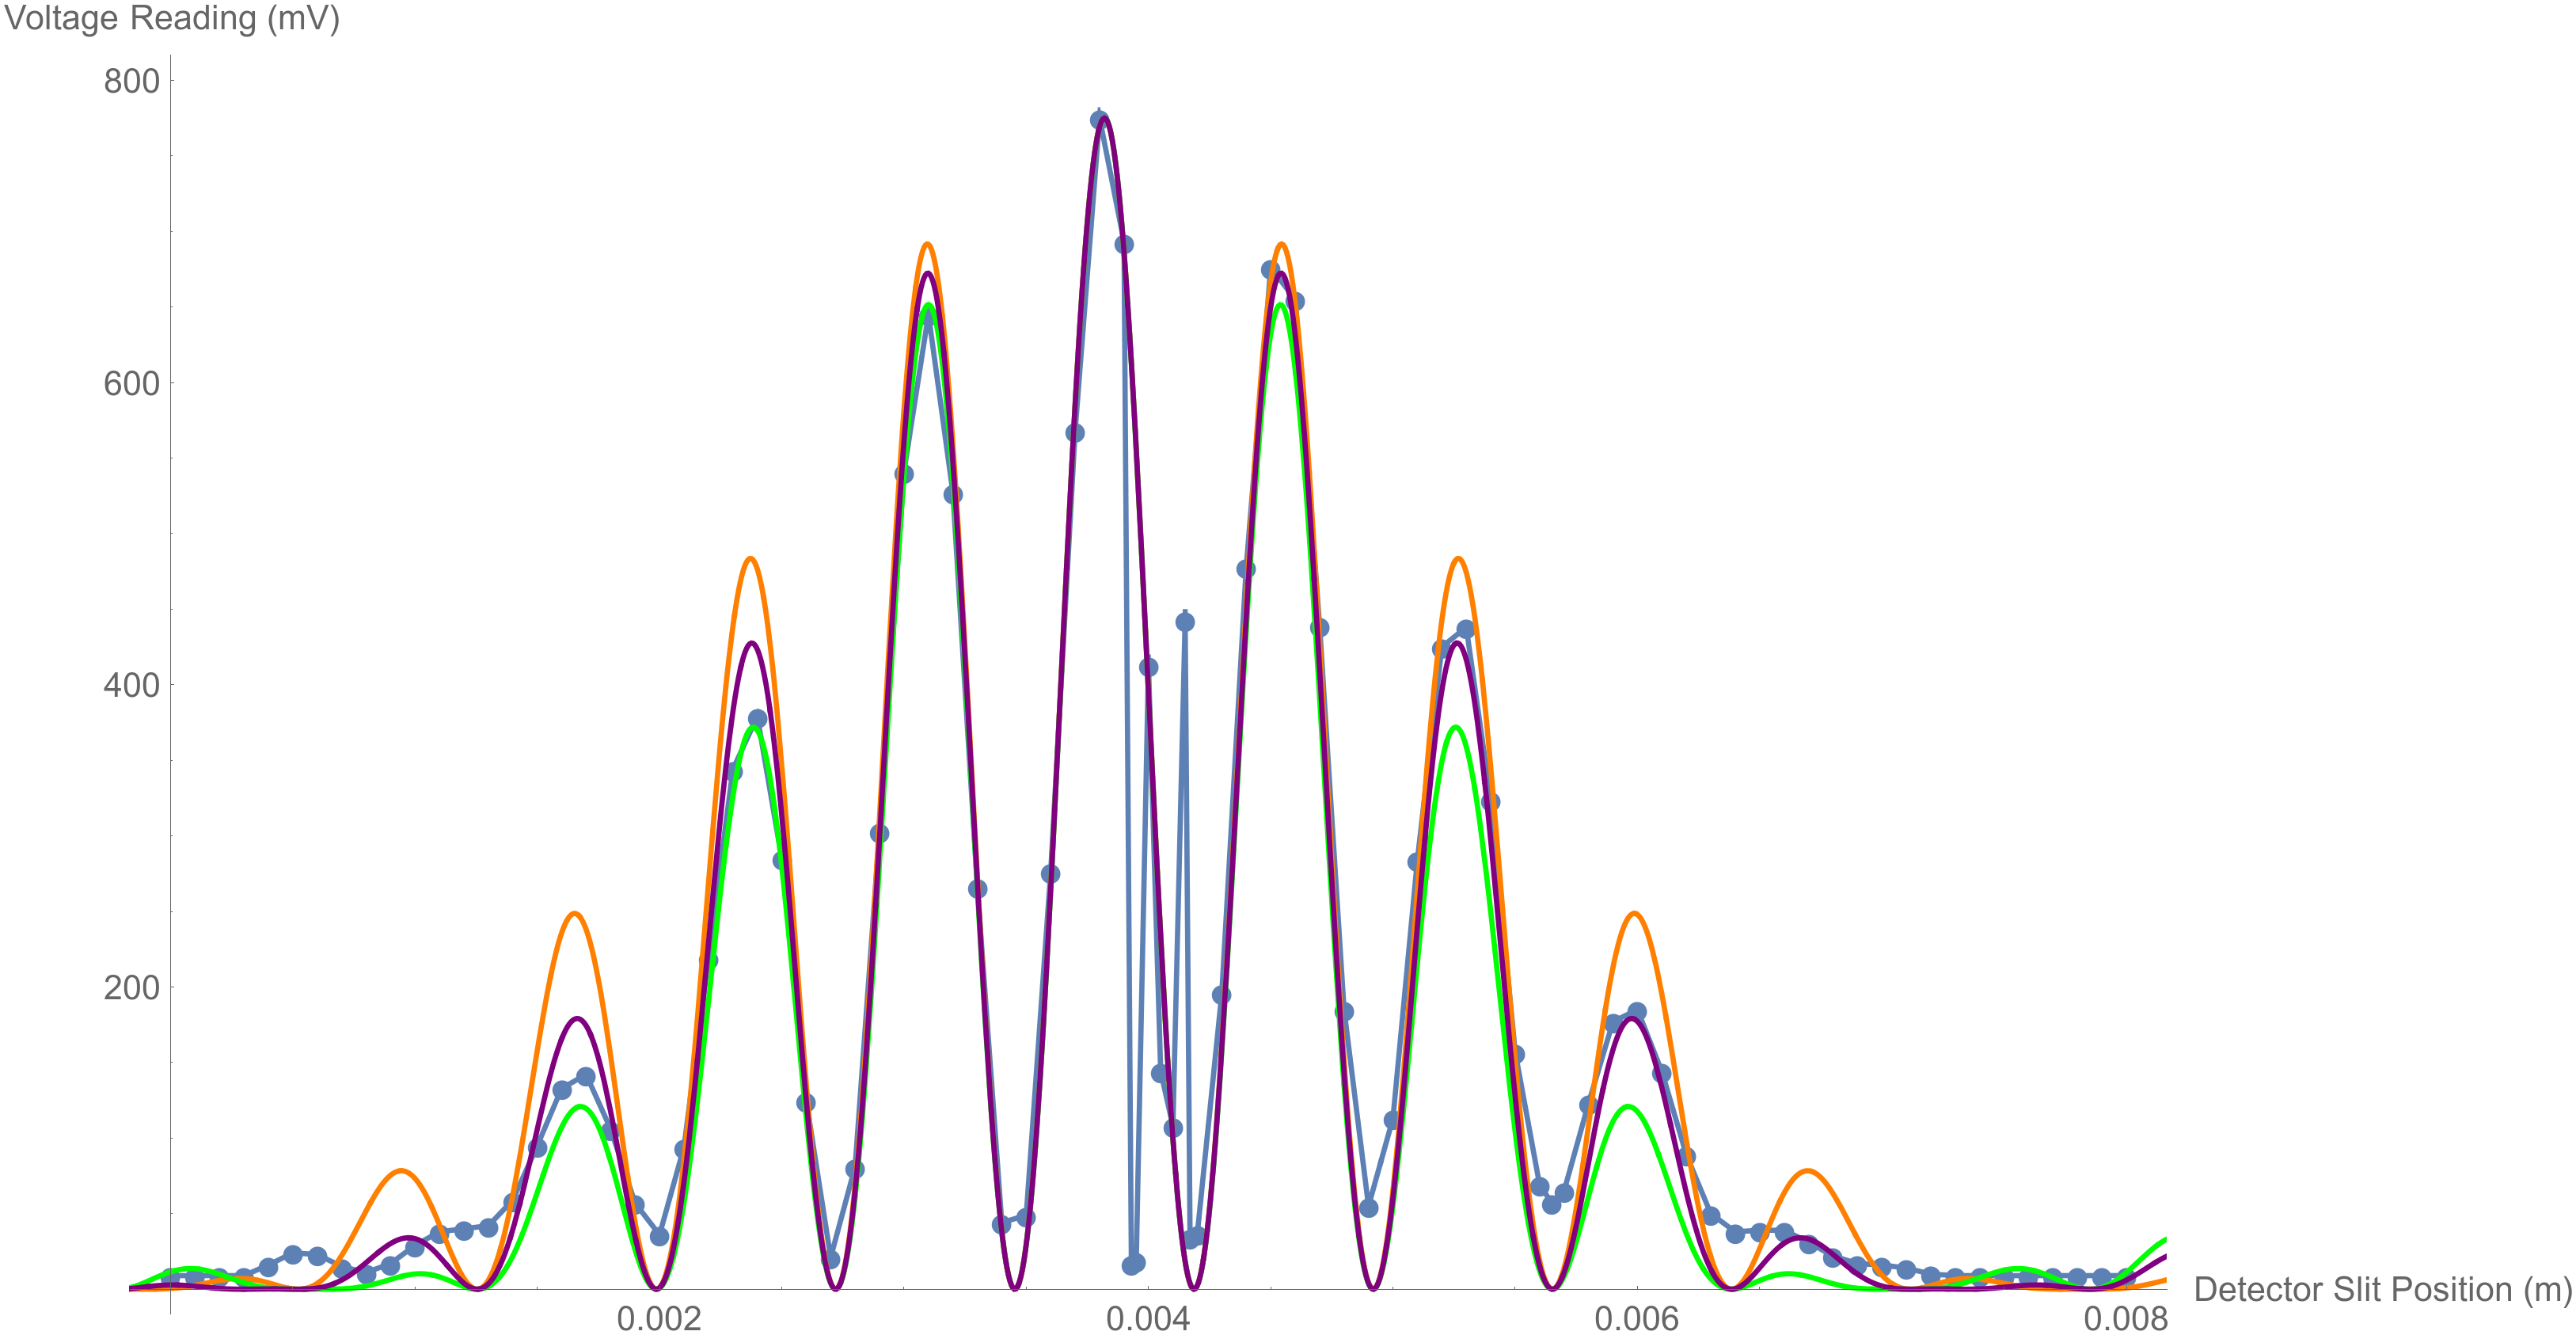
\includegraphics[width = 18cm]{wave-double-slit.png}
    \caption{\\
        Blue: Wave double slit results \\
        Orange: Expected results with \(\lambda = \SI{670}{\nano\metre}\) \\
        Green: Orange, but with \(W = \SI{0.105}{\milli\metre}\) \\
        Purple: Orange, but with \(W = \SI{0.95}{\milli\metre}\)
    }
    \label{fig:wave-double-slit}
\end{figure}
\begin{figure}
    \centering
    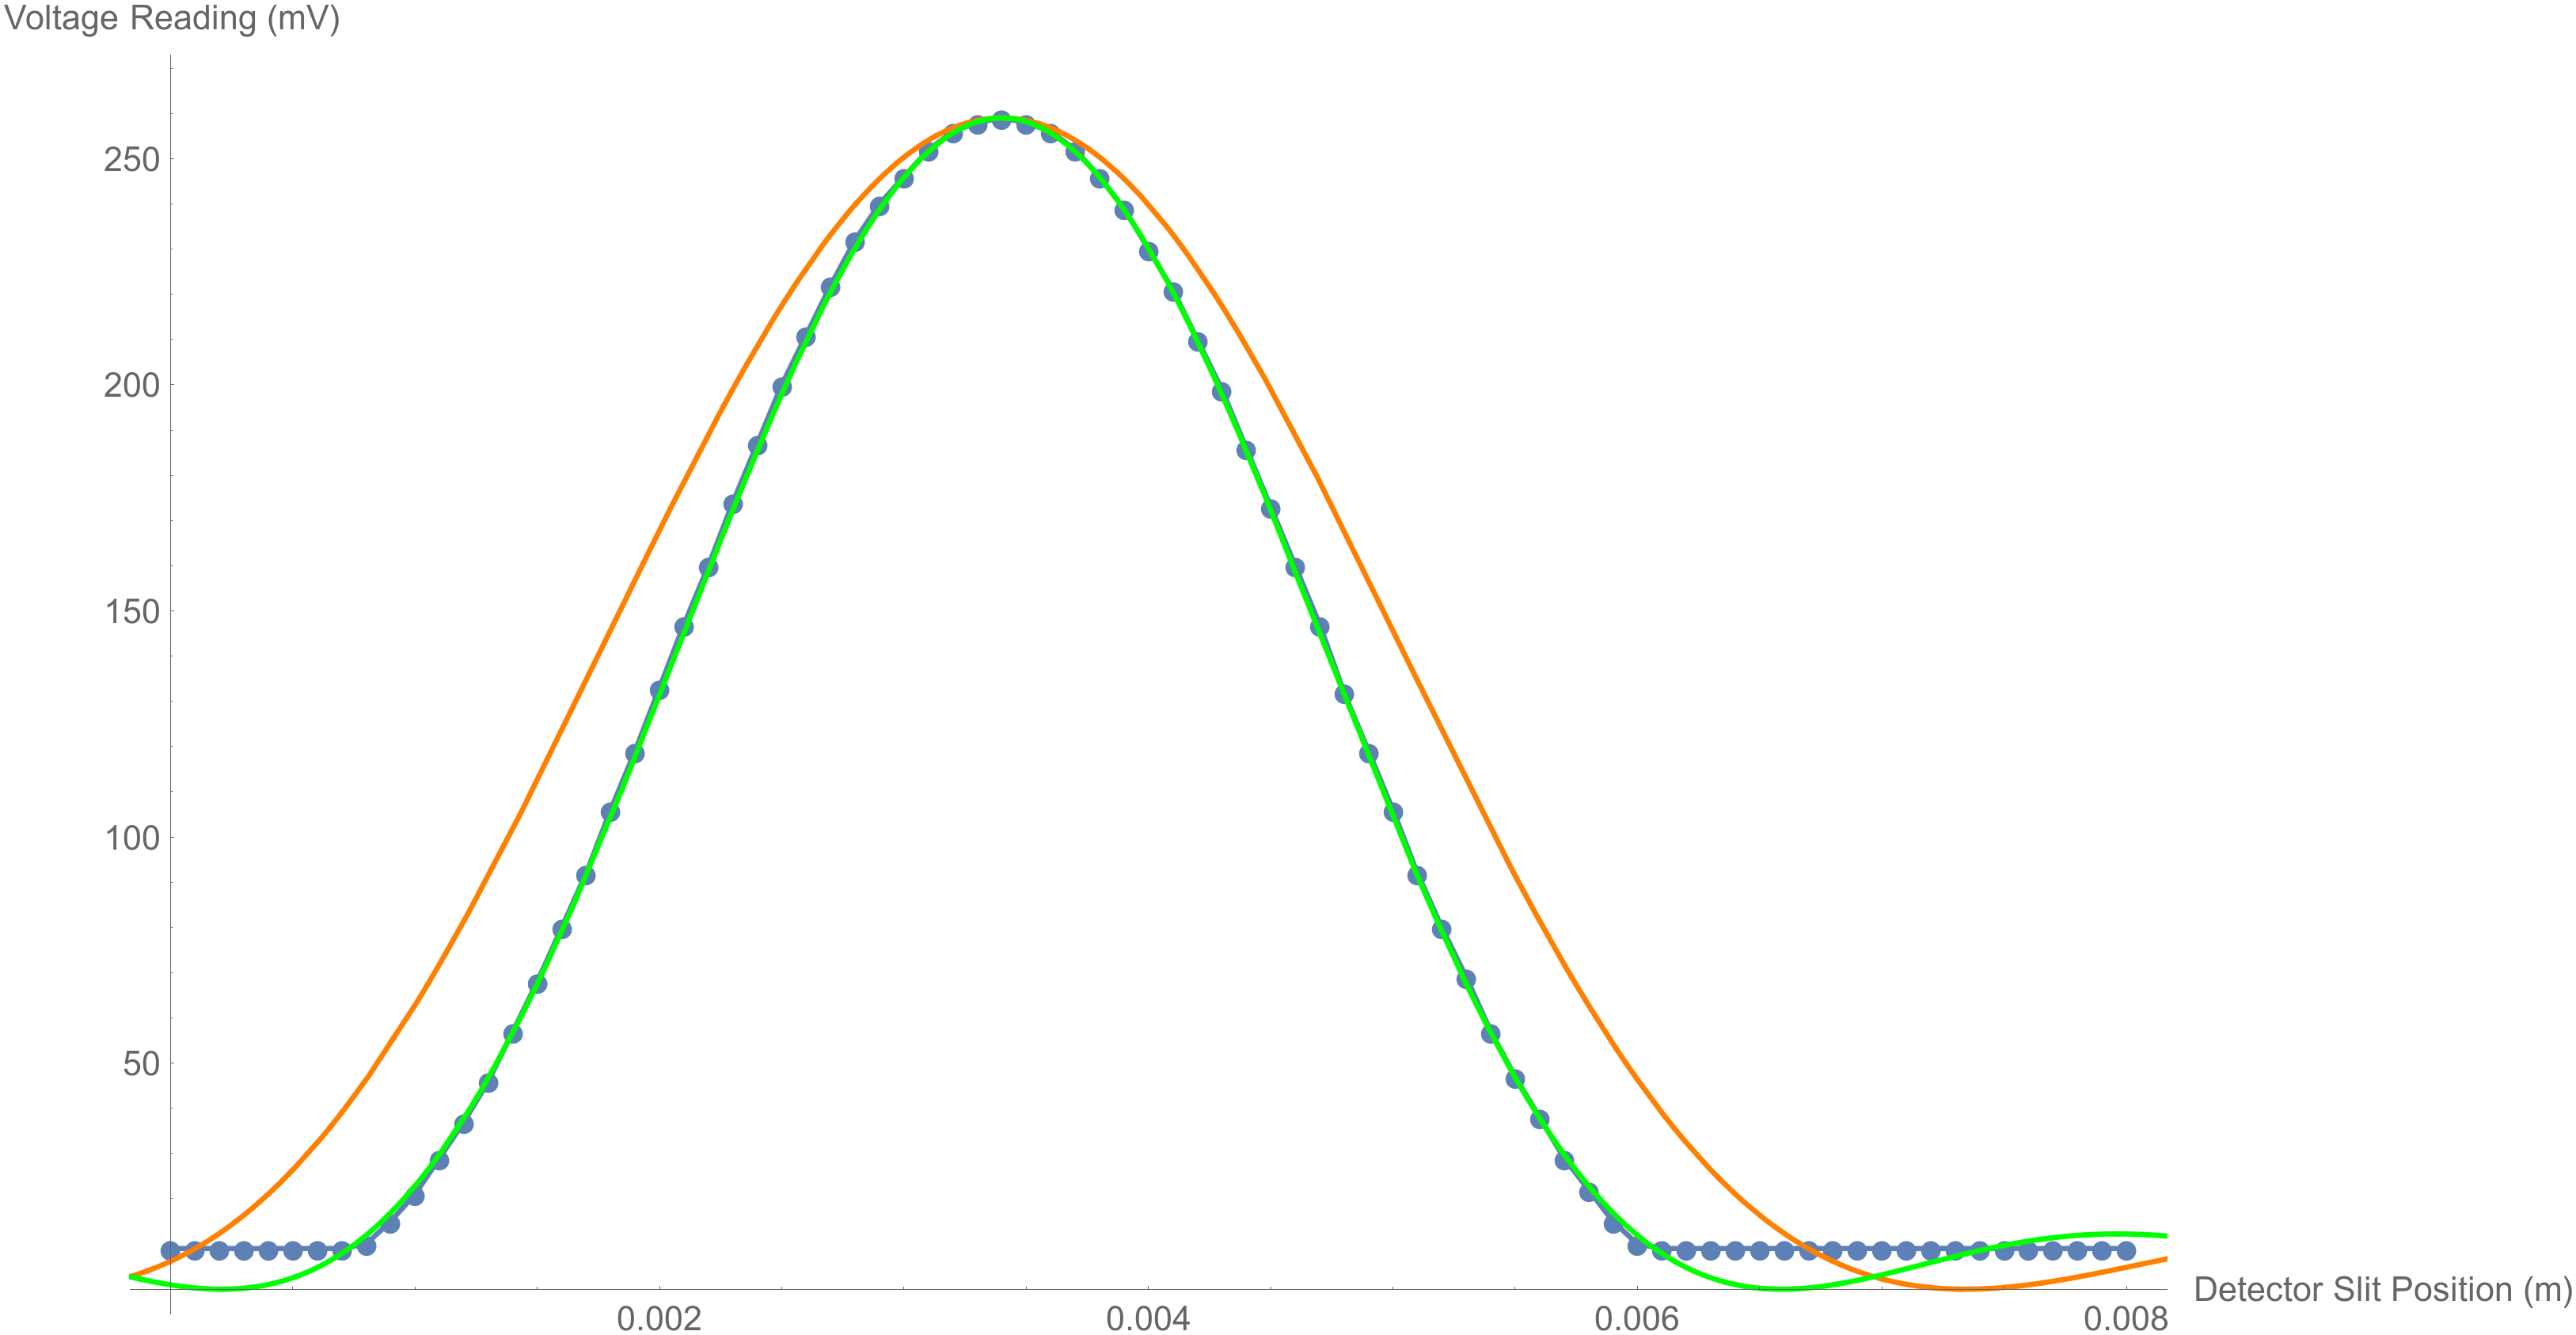
\includegraphics[width = 18cm]{wave-single-slit.png}
    \caption{\\
        Blue: Wave right slit results \\
        Orange: Expected results with \(\lambda = \SI{670}{\nano\metre}\) \\
        Green: Orange, but with \(W = \SI{0.105}{\milli\metre}\)
    }
    \label{fig:wave-single-slit}
\end{figure}

Figure \ref{fig:wave-double-slit} shows the recordings for the double slit mode, and seems okay except for some spikes around \SI{4}{\milli\metre}, which were assumed to be spurious measurements and ignored. Taking the Fourier transform revealed a peak-to-peak separation of \SI{0.74 \pm 0.09}{\milli\metre}, which corresponds to a laser wavelength of \(\lambda = \SI{6.8 \pm 0.8 e-7}{\metre}\).

Using the provided value of slit width \(W = \SI{0.085}{\milli\metre}\) resulted in too wide of a single slit diffraction envelope. Attempts to fit it optimally by modifying the slit width resulted with \(\SI{0.105 \pm 0.002}{\milli\metre}\) for the left side of the pattern, and \(\SI{0.095 \pm 0.002}{\milli\metre}\) for the right. The higher readings were weighted more for the fit to account for the increased noise of lower readings.

Figure \ref{fig:wave-single-slit} shows the recordings for the single slit mode. Notably, the maximum reading is about a third of the double slit's reading. It is also skewed to the left of the plot compared to the double slit.

Like the double slit's results, the provided slit width value produced too wide of a pattern, and a optimal fit was instead found at \(W = \SI{0.105 \pm 0.002}{\milli\metre}\).

\subsection{Particle mode}
\begin{figure}
    \centering
    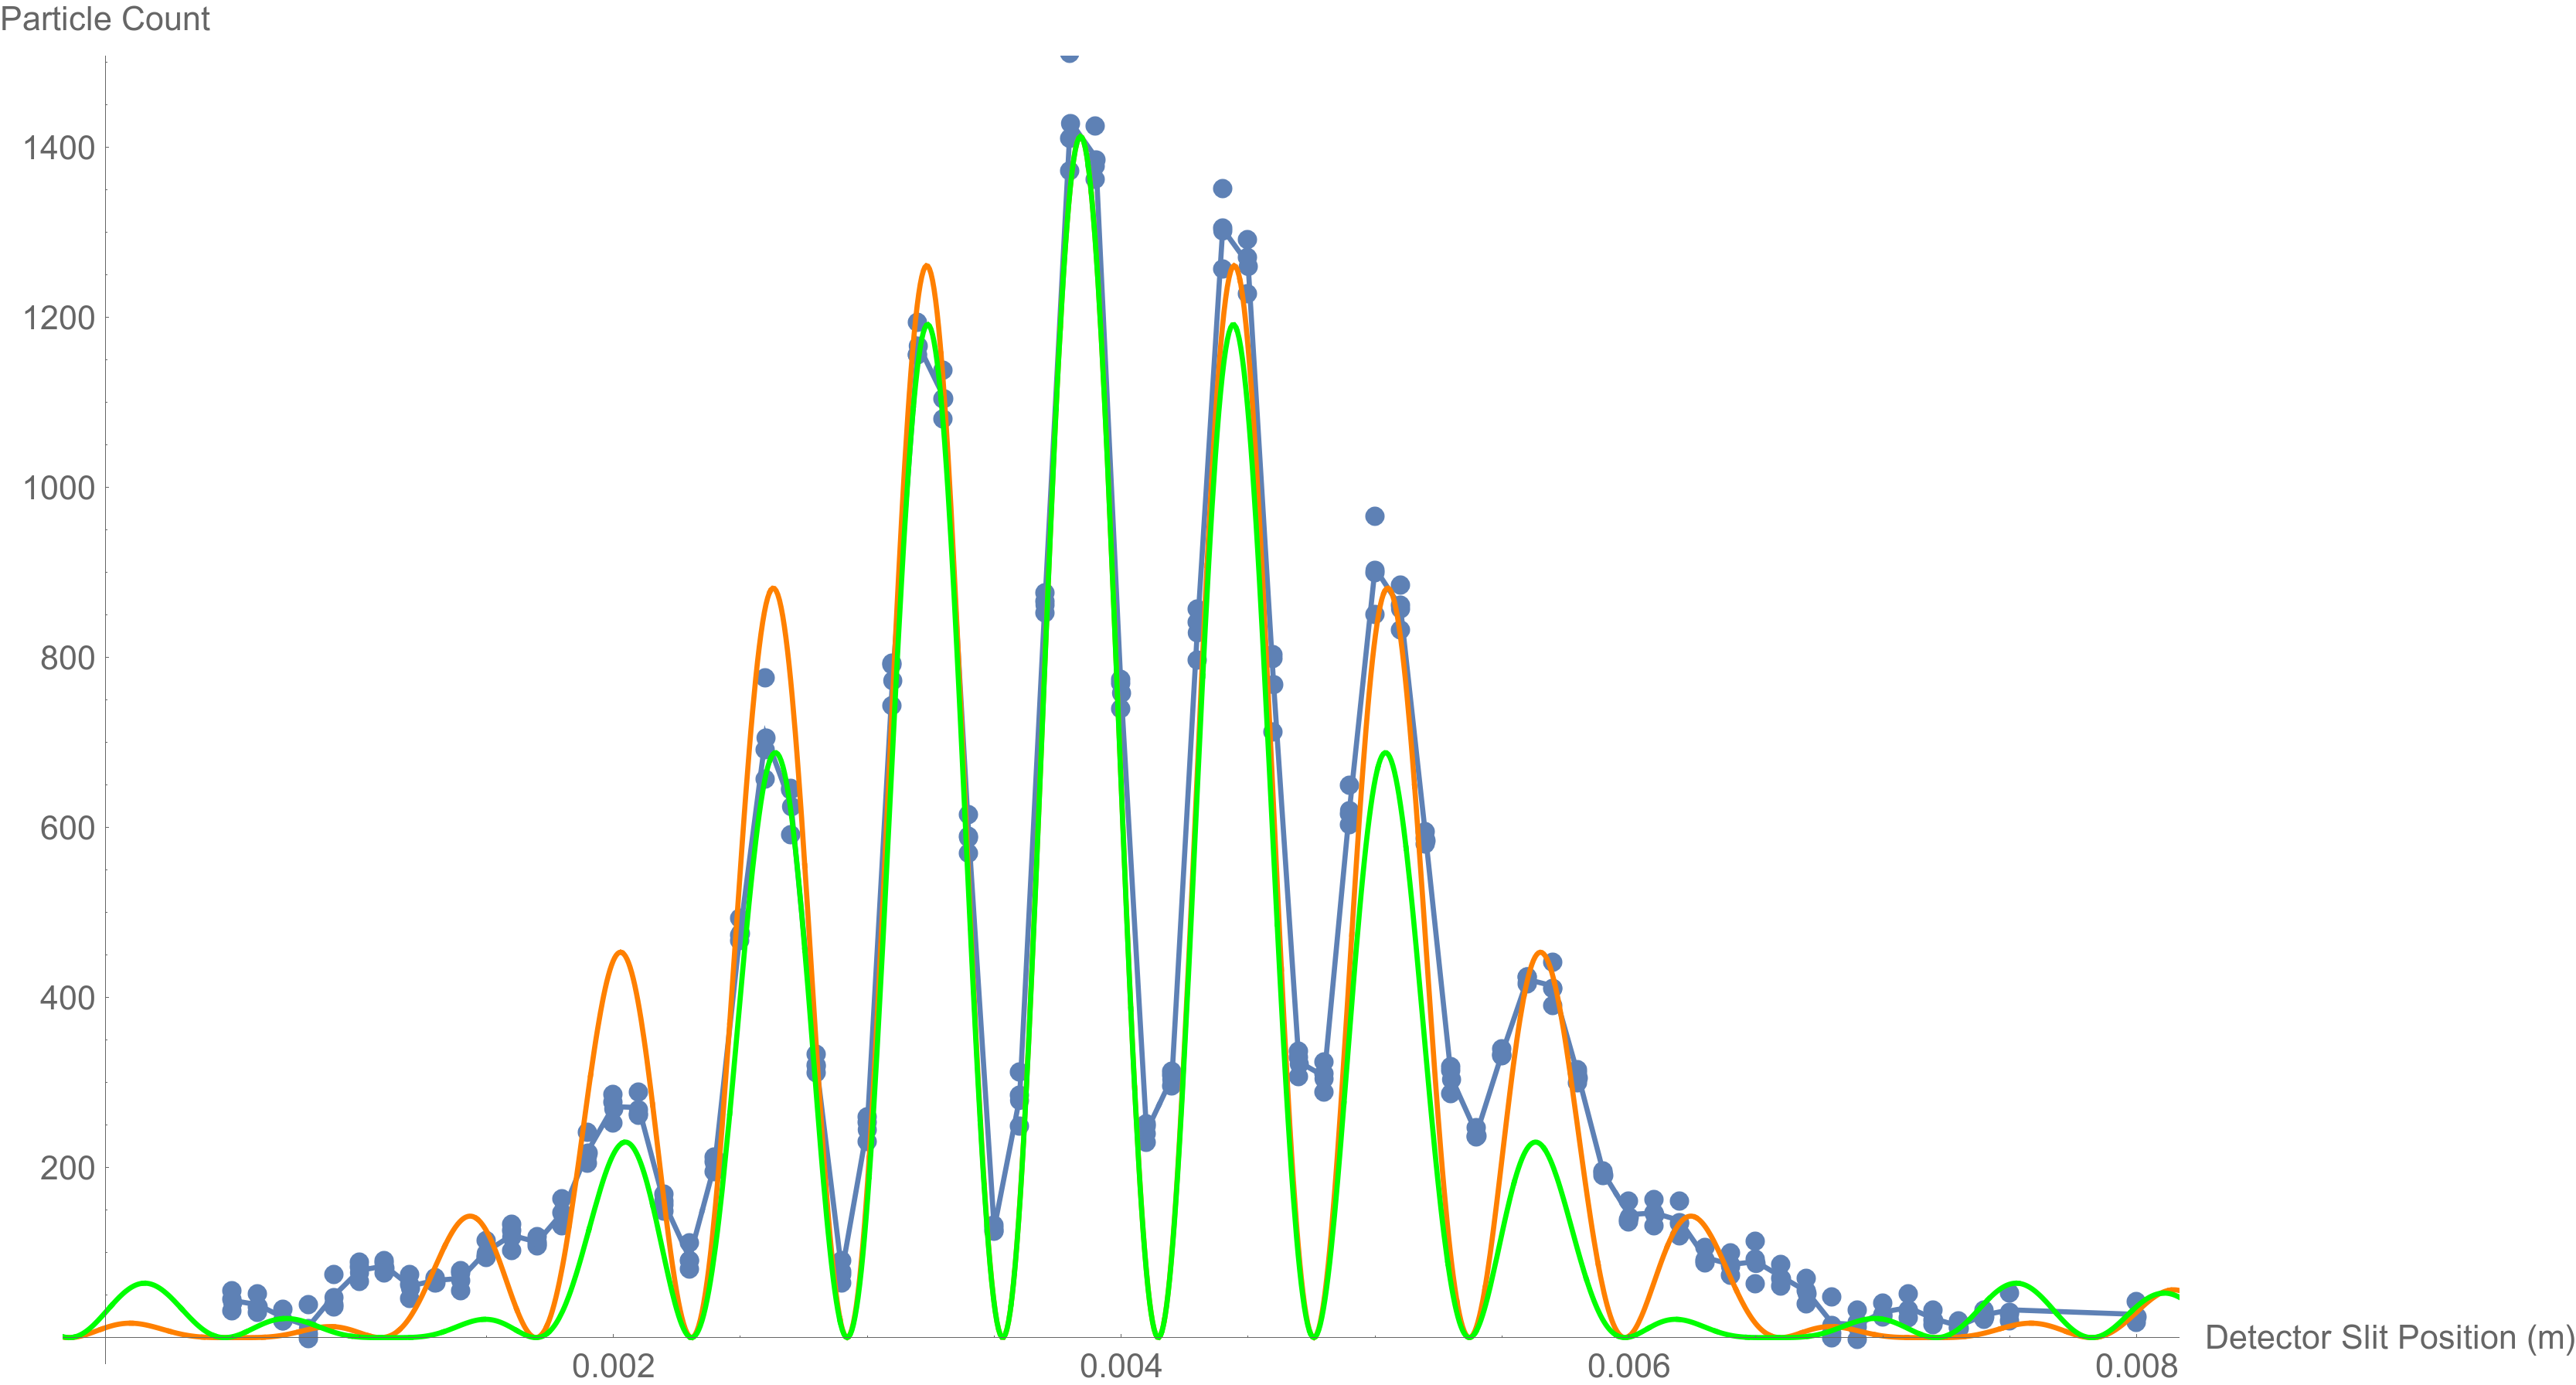
\includegraphics[width = 18cm]{particle-double-slit.png}
    \caption{\\
        Blue: Particle double slit results \\
        Orange: Expected results with \(\lambda = \SI{560}{\nano\metre}\) \\
        Green: Orange, but with \(W = \SI{0.104}{\milli\metre}\)
    }
    \label{fig:particle-double-slit}
\end{figure}
\begin{figure}
    \centering
    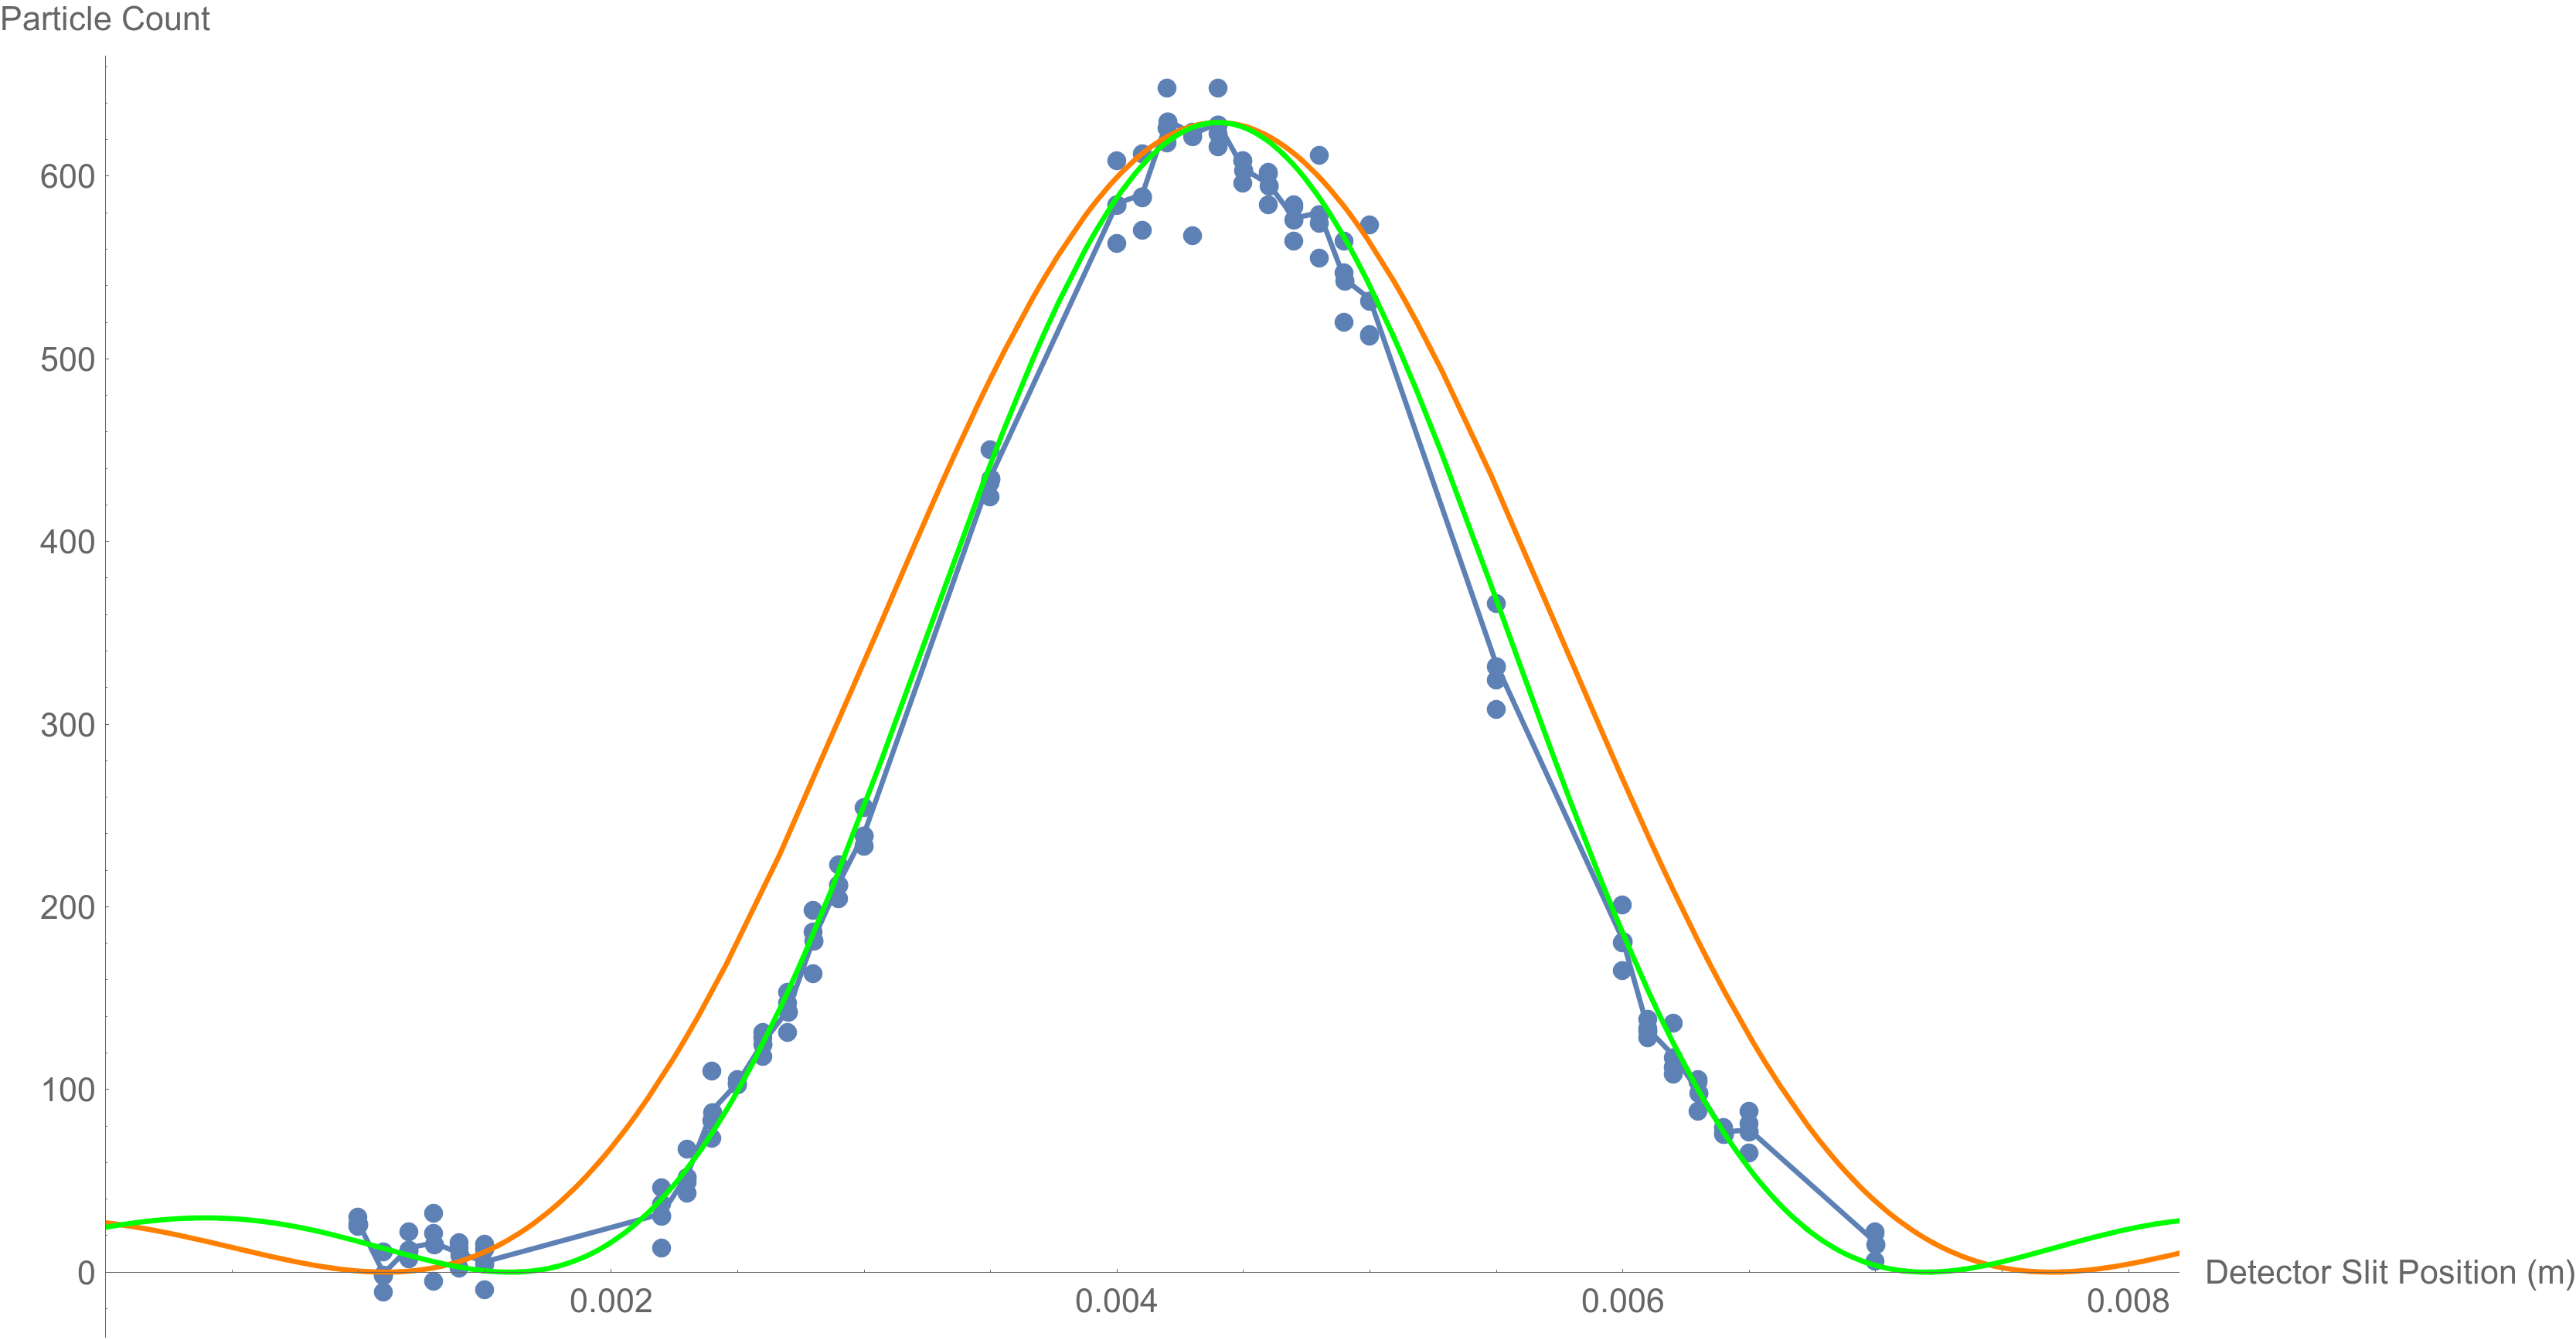
\includegraphics[width = 18cm]{particle-single-slit.png}
    \caption{\\
        Blue: Particle right slit results \\
        Orange: Expected results with \(\lambda = \SI{560}{\nano\metre}\) \\
        Green: Orange, but with \(W = \SI{0.100}{\milli\metre}\)
    }
    \label{fig:particle-single-slit}
\end{figure}

A dark current of \SI{116 \pm 5}{} was measured, and this offset was subtracted from the following results.

Figure \ref{fig:particle-double-slit} shows the recordings for the double slit mode, and it is a lot more nosier than the wave version, especially at the minima. The peak-to-peak separation was \SI{0.63 \pm 0.08}{\milli\metre}, which corresponds to a bulb wavelength of \(\lambda = \SI{5.8 \pm 0.7 e-7}{\metre}\).

Once again, the provided value of slit width \(W = \SI{0.085}{\milli\metre}\) resulted in too wide of a single slit diffraction envelope, but only on the left side. An optimal fit was instead obtained with \(\SI{0.104 \pm 0.002}{\milli\metre}\).

Figure \ref{fig:particle-single-slit} shows the recordings for the single slit mode. This time around, the maximum reading is about a half of the double slit's reading. It is also skewed to the right of the plot compared to the double slit.

Like the double slit's results, the provided slit width value produced too wide of a pattern, and a optimal fit was instead found at \(W = \SI{0.100 \pm 0.005}{\milli\metre}\).

\section{Discussion}
All the results produced the expected Fraunhofer single and double slit diffraction patterns, with only minor discrepancies. The spikes in Figure \ref{fig:wave-double-slit}, for example, are of unknown origin, and did not reappear in the other figures.

Meanwhile, the ``extra'' noisiness of the minima in the particle double slit experiment could be attributed to the wide range of wavelengths the bulb's filter allowed through (\SI{546 \pm 5}{\nano\metre}, as given by the operating instructions), hence spreading out the pattern a bit and would be noticed the most easily in the minima.

The wave mode double slit central maxima was triple that of the single slit, while only double that in particle mode. An explanation for this could be the same as the noisiness explanation as above, since the particles would be smeared out and would not achieve the same maxima.

The double slit patterns were not symmetric in intensity around the central maxima as one would expect, but this could be simply explained away as the two slits in the double slit having differing widths. This is most likely true since the given slit width of \SI{0.085}{\milli\metre} only matched half a diffraction pattern, while probable actual slit widths were \SI{0.102 \pm 0.006}{\milli\metre} and \SI{0.090 \pm 0.005}{\milli\metre}, indicating a possible wide range of widths for the equipment.

The calculated laser wavelength of \SI{6.8 \pm 0.8 e-7}{\metre} is within the expected range of red light, while the bulb's wavelength of \SI{5.8 \pm 0.7 e-7}{\metre} is also expected of green light, though its uncertainty's longer-wavelength end pushes it into orange. The bulb's wavelength also matches that of the bulb filter used to within uncertainty.

Most notably, ignoring the discrepancies listed above, the ``one particle at a time'''s pattern matched that of the wave theory of light, despite ``clearly'' being particles in the experiment. This was one of the experiments that added evidence to the quantum wave-particle duality of light (or electrons in the original experiment), where a single particle could travel down both paths and interfere with itself while still only producing a single ``particle'' reading on a detector, while revealing the diffraction pattern after averaging over time.

\end{document}
